\documentclass{standalone}
\usepackage{tikz}

\begin{document}

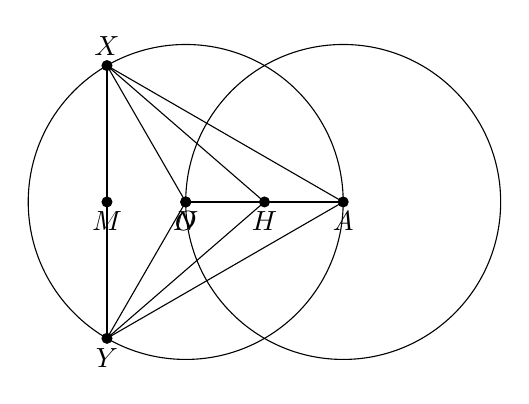
\begin{tikzpicture}[scale=2]
    % Define coordinates
    \coordinate (O) at (0,0);
    \coordinate (A) at (1,0);
    \coordinate (X) at (-0.5, 0.866);
    \coordinate (Y) at (-0.5, -0.866);
    
    % Draw circles
    \draw (O) circle (1);
    \draw (A) circle (1);
    
    % Draw lines
    \draw (O) -- (A);
    \draw (X) -- (Y);
    \draw (X) -- (A);
    \draw (Y) -- (A);
    
    % Mark points
    \fill (O) circle (1pt) node[below] {$O$};
    \fill (A) circle (1pt) node[below] {$A$};
    \fill (X) circle (1pt) node[above] {$X$};
    \fill (Y) circle (1pt) node[below] {$Y$};
    
    % Mark midpoints
    \coordinate (M) at (-0.5, 0);
    \coordinate (N) at (0, 0);
    \coordinate (H) at (0.5, 0);
    
    \fill (M) circle (1pt) node[below] {$M$};
    \fill (N) circle (1pt) node[below] {$N$};
    \fill (H) circle (1pt) node[below] {$H$};
    
    % Draw perpendiculars
    \draw (X) -- (M);
    \draw (Y) -- (M);
    \draw (X) -- (N);
    \draw (Y) -- (N);
    \draw (X) -- (H);
    \draw (Y) -- (H);
\end{tikzpicture}

\end{document}